\documentclass[12pt,preprint2]{aastex}

\usepackage{natbib, natbibspacing}
\usepackage{graphicx}
%\usepackage{setspace}
\usepackage{amsmath}
%\usepackage[small,normal,bf,up]{caption}
%\renewcommand{\captionfont}{\scriptsize}
\let\captionbox=\undefined
\usepackage[font=small,format=plain,labelfont=bf,up,textfont=it,up]{caption}
\usepackage{amssymb}
\usepackage{grffile}

\textwidth 6.5in
\partopsep 1mm
\columnsep 0.3in
\topmargin -0.25in
\setlength{\bibsep}{0.0pt}

\bibpunct{(}{)}{;}{a}{,}{,}

\shorttitle{Gravitational Instabilities and Planet Migration}
\shortauthors{Michael \& Cameron}

\begin{document}
\renewcommand{\baselinestretch}{1.00}

\title{\large TeraGrid Research Grant Proposal: The Effect of Gravitational Instabilities on Planet Migration in Protoplanetary Disks}

\author{Scott Michael\altaffilmark{1}
\and
Co-PI: Thomas Steiman-Cameron}

\altaffiltext{1}{Indiana University, University Information Technology Services, 2711 E. Tenth St., Bloomington, IN 47408,
  scamicha@iu.edu}

\begin{abstract}

  We propose to use XSEDE's unique computational and storage resources, namely large shared memory systems and wide area
  file systems, to conduct three dimensional radiative hydrodynamic simulations of protoplanetary disks with embedded
  objects. The SGI Altix UV systems in XSEDE are particularly well suited for our code, CHYMERA, because it is OpenMP
  parallel and scales to 128 cores. We also propose to continue and extend previous work under a TeraGrid research
  grant,which enabled us to utilize wide area networked (WAN) file systems to streamline our workflow and increase
  productivity. With the awarded allocation we will conduct a suite of simulations using the CHYMERA code 
  \\

\end{abstract}

\section{Planet Formation in Protoplanetary Disks}
\label{sec:intro}

There are two major theories of gas giant planet formation which are currently being considered, core accretion and disk
instability. Each theory has unanswered questions. In the core accretion picture \citep{mizuno1980}, a large solid core
must first build up through the collision of rocky materials. When this core grows to several Earth masses, it
gravitationally attracts the surrounding gas to form a gas giant planet. Observational estimates of disk lifetimes range
from 0.1 to 10 Myr, \citep{haisch2001,chen2004} with an average lifetime of $\sim 3$ Myr. Although extreme ages exist,
an upper limit of 10 Myr is generally agreed upon. Simulations by \citet{pollack1996} found that core accretion could
produce a gas giant planet $\sim 8$ Myr after kilometer-sized planetesimals have formed. However, the core masses
($M_{core}$) of the planets produced by these simulations ($\sim 15 M_{\oplus}$) are outside the range of Jupiter's core
mass (0--11 $M_{\oplus}$) inferred from the Jovian gravitational moments and detailed equation of state calculations
\citep{saumon2004}. The large range of possible $M_{core}$ is due to uncertainties in the equation of state (EOS) of
hydrogen and helium at megabar pressures. \citet{saumon2004} found the most likely values of $M_{core}$ to be $\leq 5
M_{\oplus}$. This leads to several possibilities: (1) Core accretion can occur for $M_{core} \leq 5 M_{\oplus}$, (2)
Jupiter formed with a more massive core which was then dispersed into Jupiter's outer layers, or (3) Jupiter did not
form via core accretion. More recent work by \citet{hub2005} and \citet{papa2005} have addressed the first point by
demonstrating that a gas giant planet can form via core accretion with $M_{core}=5 M_{\oplus}$ in 4.5 Myr and 3 Myr,
respectively. However, for these simulations the authors have used dust grain opacities of 2\% and 1\% of the
interstellar value. When the dust grain opacity is set to the interstellar value, gas giants form in 95 Myr and 30
Myr. Forming kilometer-sized planetesimals needed to build the cores may be difficult due the effects of
migration. Planetesimals must grow from small dust grains in the gas disk which is accreting into the central
star. Since the particles are strongly affected by gas drag until they reach sizes of tens of meters \citep{weiden1977},
they must grow to this size quickly or be accreted into the star.

On the other hand, disk instability \citep{kup1951,cam1978,boss1997} can form dense clumps via gravitational
instabilities (GIs) in times comparable to the dynamic time of the disk ($\lesssim 10^3$ yr). According to the theory,
these clumps are the self-gravitating precursors to gas giant planets. As the clump contracts, the solids contained in
the gas will rain out to form a core \citep{slattery1980}, and the clump can capture more solids from the surrounding
disk \citep{helled2006}. A protoplanetary disk must meet three main requirements to form gas giant planets via disk
instability: (1) GIs must occur in the disk, (2) the GIs must cause the disk to fragment into dense clumps, and (3)
these clumps must survive long enough to become gravitationally bound.

To parameterize the susceptibility of a disk to instability, we consider the Toomre $Q$ parameter \citep{toomre1964},
where $Q = c_s\kappa/\pi G\Sigma$. Here, $c_s$ is the sound speed, $\kappa$ is the epicyclic frequency, and $\Sigma$ the
gas surface density.
%These quantities represent stabilizing and destabilizing influences in the disk. The local pressure acts to stabilize the disk against short wavelengths while the disk rotation acts to stabilize against long wavelengths, while gravity acts to destabilize the disk. 
For $Q \leq 1$, a disk is highly unstable to an axisymmetric ring instability, and spiral instabilities set in at somewhat higher $Q$-values. Numerical simulations have found that disks with $Q$-values $\sim 1.5$ are marginally unstable \citep{boss2000,pickett2003} and that disks with $Q$-values as high as 2 can sustain instabilities. 
%As  \citet{boss2005} points out, the requirement of $Q = 1$ may lead to the erroneous conclusion that GIs cannot exist in the giant planet forming region of protoplanetary disks \citep{rafikov2005}.  

Even though spiral disturbances due to GIs may exist in a disk, they may not fragment into dense clumps. Whether a disk
will fragment is largely controlled by the cooling time. Isothermal calculations of low-Q disks, representing
instantaneous cooling, tend to form many fragments \citep{boss2000,pickett2003}. Simulations using parameterized cooling
find that the cooling times, with an adiabatic index $\gamma = 5/3$, must be less than about half an orbit time
\citep{gammie2001,rice2003b,mejia2005}. However, recent simulations have found that a disk with $\gamma = 7/5$ may
fragment with cooling times as long as two disk orbits \citep{rice2005}. Regardless of the EOS, simulations
using more realistic radiative physics find that cooling times are too long to form fragments
\citep{cai2006,cai2008,boley2006,boley2007b}. Although this position is supported by analytic arguments
\citep{rafikov2005,rafikov2007}, the fragmentation of disks with real radiative cooling remains controversial
\citep{boss2007,mayer2007,durisen2007}.

Once fragments form, they must survive long enough to become bound by self-gravity. Although many clump forming
simulations have found clump lifetimes of many disk orbits \citep{boss2003,rice2003b,mayer2004}, other
simulations find that the clumps are destroyed by the shearing motion of the disk
\citep{pickett2003,mejia2005}. Although some of this discrepancy may be due to different numerical methods
\citep{pickett2007}, simulations using the same code show clump destruction and survival also depend on the physical
conditions in the disk. Obviously the particulars of a disk (EOS, mass, temperature, opacity, etc.)
play a pivotal role in all aspects of the disk instability theory. Give the existing difficulties with both theories,
some authors have proposed hybrid theories where GIs assist planetesimal formation and accelerate core accretion
\citep{hag2003b,rice2004,durisen2005}.

\section{Gravitational Instabilities and\\ Planet Migration}
\label{sec:migration}

To date simulations published by our group have focused on the question of whether gas giant planets can form directly
via gravitational instability. We have also studied the effects of GIs on global disk properties such as surface
density, mass transport and non-axisymmetric structure. Regardless of how a gas giant planet forms, whether by core
accretion, gravitational instability, or a hybrid of the two, another interesting question is what happens to a
protoplanet after it has formed and before the disk dissipates.  Linear analysis \citep{ward1997,tanaka2002} as well as
numerical simulations \citep{nelson2003,nelson2004} indicate that in a laminar disk, or a disk dominated by MHD
turbulence, planets tend to migrate inward rapidly via Type I or Type II migration, depending on their mass, and are
accreted onto the central star within a few $\times 10^5$ years. In the case of Type I migration, the protoplanet is not
massive enough to open a gap in the disk and migrates inward by exchanging angular momentum with the disk via
gravitational torques. With Type II migration the protoplanet is massive enough to open a gap and then migrates with the
motion of the surrounding disk. In either case, the timescale for the protoplanet to migrate into the central star is
very short compared to disk lifetimes. However, if the disk is gravitationally unstable, the instabilities may slow
inward migration, or even cause the protoplanet to move outward. This would help to explain how protoplanets can survive
in a protoplanetary disk after they form as well as provide insight into their distributions in multiple planet systems,
26 of which have already been discovered. So far, migration in gravitationally unstable disks has only been studied in
the context of fragmented disks \citep{mayer2004,boss2005}.

Additions made to our code prior to our 08-09 award allowed us to follow the motion of massive particles in
protoplanetary disks undergoing GIs. We were also able to model the effect of a massive planet on the disk and the
feedback between the planet and GIs. By examining a range of masses ($0.3 M_{\mathrm{jup}}$ -- $3 M_{\mathrm{jup}}$), we
have been studying how GIs affect gap opening and the transition between Type I and Type II migration.

\section{Computational Methodology}
\label{sec:method}

The equations of hydrodynamics and self-gravity are:
\begin{eqnarray}
\frac{\partial \rho}{\partial t} + \nabla \cdot \rho \boldsymbol{v} & = & 0,\label{massconteq}\\
\frac{\partial \rho \boldsymbol{v}}{\partial t} + \nabla \cdot \rho \boldsymbol{vv} & = & -\nabla p - \rho \nabla \Phi_{\mathrm{tot}}\nonumber\\
&& - \nabla \cdot (\rho \mathsf{Q}),\label{motioneq}\\
\frac{\partial \epsilon}{\partial t} + \nabla \cdot \boldsymbol{v} \epsilon & = & - p \nabla \cdot \boldsymbol{v} + \Gamma - \Lambda,\label{energyeq}\\
\nabla^2 \Phi_{\mathrm{disk}} & = & 4 \pi G \rho\label{graveq}.
\end{eqnarray}
These are the mass continuity equation \eqref{massconteq}, the equation of motion \eqref{motioneq}, the internal energy equation \eqref{energyeq}, and Poisson's equation \eqref{graveq}. Here $\rho$ is the mass density, $\mathbf{v}$ represents the gas velocity, $p$ is the gas pressure, $\mathsf{Q}$ is the artificial viscosity tensor, $\epsilon$ is the internal energy density, $\Gamma$ represents heating due to artificial viscosity, $\Lambda$ represents net cooling due to energy transport via radiation or other mechanisms, and $\Phi_{\mathrm{tot}}$ and $\Phi_{\mathrm{disk}}$ are the total and disk gravitational potentials, respectively.

The Indiana University Hydro Group (IUHG) code, CHYMERA, is an Eulerian scheme which is second order in both space and
time. The equations are evolved in cylindrical coordinates ($\varpi$,$\phi$,$z$) on an evenly spaced three dimensional
grid. The rotation axis of the disk is aligned with the $z$-axis. The disk is treated as having reflection symmetry about
the midplane in order to reduce computation time. Poisson's equation is solved via Fourier decomposition and cyclic
reduction \citep{tohline1980}. Shock heating is modeled via artificial viscosity \citep{pickettphd1995} and radiative
cooling is treated by a method outlined in the following section. Artificial viscosity is treated using a von
Neumann-type scheme \citep{norman1986} in which the off-diagonal terms of the artificial viscosity tensor are set to
zero and the heating due to artificial viscosity is given by
 \begin{equation}
 \Gamma = \rho(\mathsf{Q}_{rr}\partial_r v_r + \mathsf{Q}_{\phi\phi} r^{-1}\partial_\phi v_\phi + \mathsf{Q}_{zz} \partial_z v_z). 
\end{equation}

\subsection{Cooling Algorithm}
\label{sec:cooling}

The cooling algorithm used in CHYMERA, as implemented by \citet{boley2007b}, is a radiative routine where the transport
of energy by radiation in the vertical direction is computed using the method of discrete ordinates
\citep{chandra1960}. Here each vertical column is considered to be a separate plane parallel structure, and the transfer
is calculated using a single upward ray at $\mu = 1/\sqrt{3}$ to the vertical and a single downward ray at $\mu =
-1/\sqrt{3}$, where $\mu$ is the cosine of the angle between the ray and the disk vertical . For optical depths greater
than $\tau = 1/\sqrt{3}$, transport in the $\varpi$ and $\phi$ directions is treated using flux-limited diffusion. No
transport is modeled in the $\varpi$ and $\phi$ directions for $\tau < 1/\sqrt{3}$. The advantage of this scheme is that
the vertical transport is modeled explicitly, no fitting of an atmosphere is required and cell-to-cell coupling is
included explicitly for all $\tau$.

\subsection{Planet Integrator}
\label{sec:planetintegrate}

In order to model the effect of GIs on the migration of protoplanets and planets, routines have been added to the
standard version of the code to follow the motion of massive particles in a GI-active background. The simplest
second-order accurate scheme to implement is the leapfrog scheme, sometimes known as the Verlet method. It has been
shown to be the simplest example of a symplectic integrator \citep{channell1990,yoshida1990} and produces high accuracy
and stability when compared with other second-order integrators such as Runge-Kutta methods. Generally the equations are
written in a time-interleaved fashion with the positions $\boldsymbol{r}$ and accelerations $\boldsymbol{a}$ specified
on the integer time steps and the velocities $\boldsymbol{v}$ specified on the half-integer steps as in
\begin{subequations}
\label{leapfrog}
\begin{eqnarray}
\boldsymbol{r}_1 &=& \boldsymbol{r}_0 + \boldsymbol{v}_{1/2} \Delta t\\
\hspace{-.25in} \mathrm{and} \hspace{.25in} \boldsymbol{v}_{3/2} &=& \boldsymbol{v}_{1/2} + \boldsymbol{a}_1 \Delta t.
\end{eqnarray}
\end{subequations}
Note that the displacement of $\boldsymbol{v}$ with respect to $\boldsymbol{r}$ and $\boldsymbol{a}$ is time symmetric, preventing the accumulation of error in the energy over time.

\subsection{Code Testing}
\label{sec:tests}

Extensive testing of the hydrodynamic routines and radiative routines has been performed by several researchers in the
IUHG \citep{yangphd1992,pickettphd1995,pickett2000,pickett2003,mejia2005,boley2007b}. In order to test the planet
integration and interpolation algorithms included in the code, simulations were performed in which an initial
axisymmetric disk was held fixed while a planet orbited in its potential. Since the mass distribution of the
protoplanetary disk used is not a simple one, results could not be compared to analytic solutions. However the $z$
component of the angular momentum was conserved to one part in $10^{13}$ and the expected rosette pattern was observed
in the orbit, which maintained nearly constant apapse and periapse radii.

\section{Previous Work and Planned Simulations}
\label{sec:plan}

\subsection{Studies in Planet Migration} \label{sec:migplan}

Many gravitationally unstable protoplanetary disk studies have been carried out under previous TeraGrid awards granted
to PI Richard H. Durisen. Namely, TeraGrid awards TG-AST080031T and TG-AST090027, which resulted in several publications
\citep{henschel2010,michael2010a,michael2010b,michael2011a} in both the astronomical sciences and in computer
science. With the current request for XSEDE, we plan to extend and expand upon this work. Under PI Scott Michael, we
have already received a startup award (TG-AST110027) that has been put to great use, allowing for benchmarking of the
code on the new Altix UV architecture and submission of an article to Astrophysical Journal Letters, a peer-reviewed
express scientific journal that allows astrophysicists to rapidly publish short notices of significant original research
\citep{michael2011b}. Under our previous awards we planned to study the effect of both planet mass and planet position
on migration in a GI-active disk. Subsequently we realized an additional interesting study would be to understand the
effect a planet might have on a marginally stable disk. For this reason we undertook a series of seven simulations to
study the effects of planet mass and the effect of injecting the planet at different times in the evolution of the
disk. Figure \ref{fig:modes} is an example from one such simulation.

We plan to continue our work and follow up our studies on planet mass with studies of injection position in an already
GI-active disk. Our current studies of GI-active disks have placed planets of varying mass at the co-rotation radii of
the dominant GI active modes. We will follow up on these studies by injecting varying mass planet outside the
co-rotation radii of the dominant modes to determine under what conditions outward migration might be possible. By
placing the planet at the outer Linblad resonance of the strongest mode \citep{binney1987}, we hope to understand how
sensitive the planet's motion is to its location relative to the dominate GI modes and when its direction can change.

One interesting result of work conducted under the previous award was the finding that upon injecting planets at the
beginning of our simulations, the presence of the planet affects the onset of GI activity causing the co-rotation of the
dominant mode to shift outward. We will conduct further tests by injecting planets at different locations at the
beginning of the simulations to study how the planet's initial position affects the onset of GIs.

\begin{figure} [t] % t=top, b=bottom, h=here, p=separate page
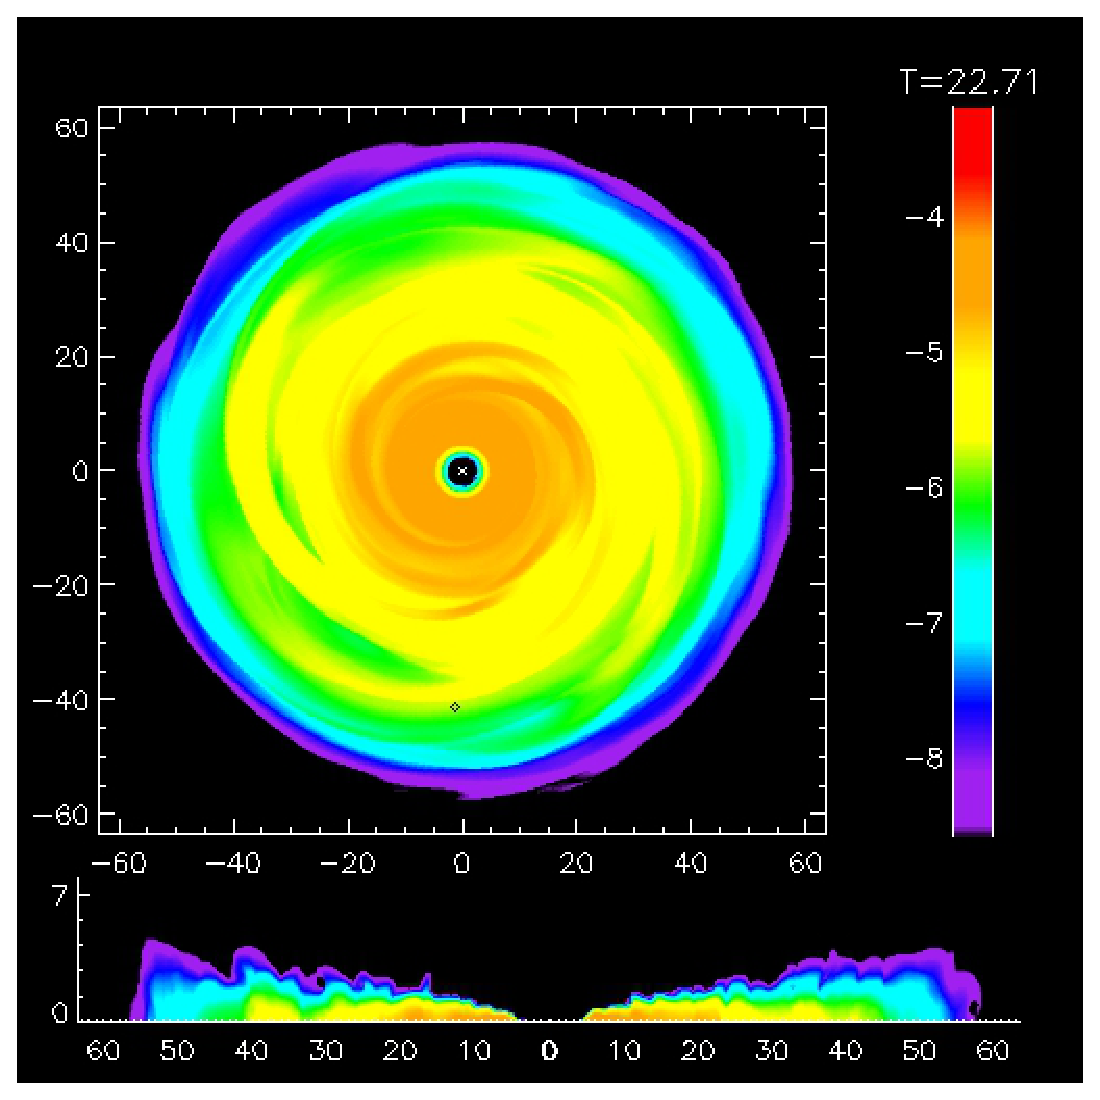
\includegraphics[width=0.47\textwidth]{0.3JUP.eps}
\caption{Midplane density map of a simulation of a gravitationally unstable disk with a 0.3 Jupiter mass planet inserted
  at 10.5 ORP. By 22.7 ORP the planet has migrated outward from its initial position of 25 AU. Axes are labelled in AU
  and the density scale is logarithmic. The white X indicates the position of the system COM in the accelerated frame,
  and the black diamond indicates the position of the planet. \label{fig:modes}}
\end{figure}

Estimates for the resolution requirements were based on the planet's Hill radius. In order to capture the gravitational
effect of the planet, one would like to resolve the Hill sphere with many resolution elements, at minimum one resolution
element in 25 per cent of the Hill sphere. So ideally we would have,
\begin{equation}
\Delta \phi \varpi = 0.25\varpi \sqrt[3]{\frac{m_{\mathrm{planet}}}{3M_{\mathrm{star}}}}.
\end{equation}
For our least massive planet this gives a $\phi$-resolution of $~ 520$ resolution elements. We have conducted
simulations using a resolution of 512x512x64 ($\varpi$,$\phi$,$z$) with this planet mass and have not detected any
numerical effects due to inadequate resolution. We will continue to use this resolution for our further simulations,
which will include two simulations studying planet position in a GI-active disk, two simulations studying the effect of
planet injection position in an initially GI-inactive disk, and several simulations studying circumbinary disks. In
total we plan 5 simulations at this resolution each of which should be evolved for 10--20 ORPs which is roughly equal to
1--2 million time steps.

\section{Performance and Scalability}
\label{sec:performance}

Our previous estimates for the needed SUs were based on extrapolation from smaller core counts. Extensive testing of the
code's scalability on several Altix machines has been conducted under the previous award's ASTA component. To date, we
have evolved an aggregate of ~4 million production time steps and 1-2 million time steps in testing and development,
these efforts have consumed 300,000 SUs. These real measurements have shown that a 2 million time step simulation will
require $\sim\!\!100,000$ SUs which is a factor of two greater than our initial estimate. In total, to complete the 5
simulations we are planning, we request 500,000 SUs on the Altix at PSC, Pople.

\section{Summary}
\label{sec:summary} 

We seek to carry out a suite of numerical simulations to study the effects of GIs on planetary migration. These
simulations would take a prohibitively long time using our currently available resources. In order to carry out our work
in a reasonable amount of time, we request 500,000 SUs of computer time on PSCs Pople, and 1 year of advanced support to
help with parallelization and development of automated workflows.

\scriptsize
\setlength{\baselineskip}{7.5pt}
\setlength{\bibspacing}{\baselineskip}

\bibliographystyle{apj}
\bibliography{general}



\end{document}










